% !TeX root = ..\main.tex

\section{Neo4j Features} \label{sec:features}

In this section we will discuss the features of Neo4j.


\subsection{Cypher} \label{subsec:Cypher}

Cypher is the query language of Neo4j. It is a declarative language, which means that you describe what you want to achieve, but not how it should be done. As it is a graph query language, it is designed to work with graph data structures. On the first look it has similarities with ASCI-art.

\begin{figure}[!h]
    \centering
    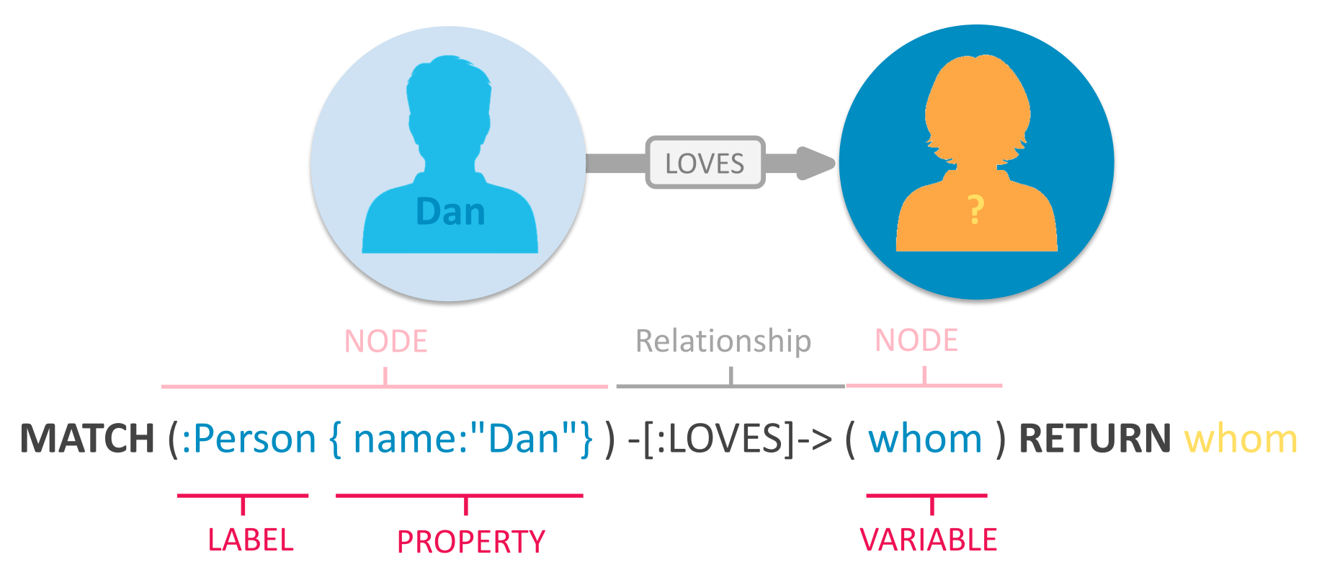
\includegraphics[width=1 \linewidth]{images/cypher_example.png}
    \caption{Cypher Query Language Basics \parencite{neo4j:cypher}} \label{img:cypher}
\end{figure}

In the example in Figure \ref{img:cypher} you can see the basic structure of a Cypher query. It starts with a “MATCH” statement, which is used to find the nodes and relationships you want to work with. Nodes are represented by round brackets and relationships by square brackets with ASCI-art like arrows to show the direction of the relationship. Inside those brackets you can specify the labels of the nodes and the type of the relationship. Additional properties can be specified with curly brackets. In this example the second node in the query has a variable name, which is used to refer to it in the following statements. After the “MATCH” statement you can specify the “RETURN” statement, which is used to return the results of the query. In this example the “RETURN” statement returns the variable name of the second node.


% %%%%%%%%%%%%%%
\todo{}
Uses Query Language called Cypher which I will explain in depth in the following
It offers Native drivers for most popular programming languages
Neo4j is also designed for the Cloud, with a focus on both vertical and horizontal scalability.
Optimizations like in-memory graph processing, enables it to efficiently handle complex graph data structures.
- It outshines relational databases in query performance by orders of magnitude
Additionally, Neo4j built-in support for clustering and replication allows it to seamlessly scale horizontally

